\documentclass[11pt, ngerman, fleqn, DIV=15, headinclude, BCOR=2cm]{scrreprt}

\usepackage{../../header}

\usepackage{placeins}
%\usepackage[maxfloats=50]{morefloats}

\usepackage{csquotes}

\usepackage{tikz}
\usetikzlibrary{chains}
\usetikzlibrary{shapes.geometric}

\tikzset{device/.style={
                rectangle,
                minimum size=6mm,
                draw=black
            },
            monitor/.style={
                rectangle,
                rounded corners=2mm,
                minimum size=6mm,
                draw=black
            },
        }

\usepackage{pgfplots}
\pgfplotsset{
    compat=1.9,
    width=0.8\linewidth,
    xticklabel style={/pgf/number format/use comma},
    yticklabel style={/pgf/number format/use comma},
}
\usepgfplotslibrary{polar}

\usepgfplotslibrary{external}
\tikzexternalize[mode=list and make]
\tikzsetexternalprefix{Abbildung-}

\DeclareSIUnit{\skt}{SKT}

\usepackage{booktabs}

\usepackage{subcaption}

\hypersetup{
    pdftitle=
}

\subject{Praktikumsprotokoll}
\title{Driftkammer}
\subtitle{Versuch P515 -- Universität Bonn}
\author{
	Frederike Schrödel \\
	\small{\href{mailto:fschroedel@gmx.de}{fschroedel@gmx.de}}
	\and
	Simon Schlepphorst \\
	\small{\href{mailto:s2@uni-bonn.de}{s2@uni-bonn.de}}
}

\date{2015-11-02}

\publishers{Tutor: Dr. Jürgen Hannappel
}

\begin{document}

\maketitle

\begin{abstract}
Ziel des Driftkammerversuches ist es, die Funktionsweise und Datengewinnung aus einer Driftkammer zu verstehen.
Hierzu nehmen wir dem Prototyp einer Driftkammer in Betrieb, 
bestimmen dessen Ansprechverhalten bei verschiedenen Hochspannungen mit oder ohne Bestrahlung durch ein $\beta$-Strahler  
und ermitteln seine Orts-Driftzeitbeziehung.
\end{abstract}

\tableofcontents

\chapter{Theorie}

\section{Einführung}
In der modernen Physik spielen Teilchenbeschleuniger eine wichtige Rolle und 
mit ihnen auch verschiedene Teilchendetektoren.
Wir beschäftigen uns im folgenden mit einer Driftkammer als Beispiel für einen 
gasbasierten Teilchendetektor.
Im Gegensatz zur Nebelkammer lässt sich der Durchgangsort ionisierender
Strahlung in einer Driftkammer elektronisch auslesen.
In diesem Versuch werden die charaktristischen Eigenschaften des Prototypen 
einer Driftkammer des BGO-OD-Experimentes untersucht.
Hierbei wird zum einen das Verhalten der Driftkammer mit und ohne
Strahlungsqulle ($^{90}\text{Sr}$-Präperat) unter verschiedenen Parametern verglichen.
Außerdem wird eine Langzeitmessung ohne Präperat durchgeführt, bei der die 
Winkelverteilung der kosmischen Strahlung vermessen wird.

\section{Theorie}
\subsection{Aufbau der Driftkammer}
Die Driftkammer besteht aus einer mit Argon-Kohlenstoffdioxidgemisch 
(im Verhältnis $ 82\%-18\% $) gefüllten Kammer, welche mit Drähten durchspannt
ist. Hierbei bilden jeweils sechs hexagonal angeordnten Potentialdrähte, an
denen eine hohe negative Spannung anliegt, und der in der Mitte liegede geerdete 
Anodendraht eine Driftzelle.
Die Potentialdrähte erfüllen hierbei die Aufgabe ein zylindrisches Feld zu 
erzeugen. Dieses soll die, durch Ionisierung frei werdenen Elektronen in die 
Richtung des Anodendraht zu beschleunigen und verhindern, dass das Elektron in 
einer anderen Zelle detektiert wird.
Die Spannung der Potentialdrähte kann von \SIrange{0}{3000}{\volt} variiert werden.

\begin{figure}
	\centering
	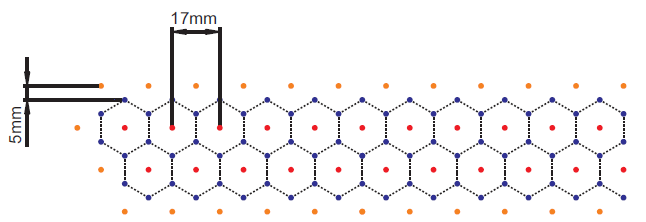
\includegraphics[width=\linewidth]{../Driftkammer.png}
	\caption{%
		Anordnung der Drähte in der Driftkammer
		%TODO Quelle angeben
	}
	\label{fig:aufbau_driftkammer}
\end{figure}

Ordnet man die einzelnen Driftzellen wie in
Abbildung~\ref{fig:aufbau_driftkammer} an, so erhält man eine Driftkammer.
Um das Verhältnis der Gaszusammensetzung, dessen Druck und Temperatur möglichst
konstant zu halten, wird das Gasgemisch kontinuierlich getauscht.
Denn diese Rahmenbedingungen entscheiden mit über die Driftgeschwindigkeit der
Elektronen.
Um durch die Driftgeschwindigkeit nicht durch die Bewegung des Gases zu
verfälschen, läuft der Gasaustausch sehr langsam ab.

\subsection{Ionisation der Gasatome}
Für schwere geladene Teilchen lässt sich der Energieverlust durch
Primärionisationen in der Driftkammer durch die Bethe-Bloch-Formel beschreiben.
\[
    -\dod Ex = \frac{4 \pi r^2_e m_e c^2 N_\text{A} Z z^2}{A \beta^2}\sbr{\ln\sbr{\frac{2m_e c^2 \beta^2}{(1-\beta^2)I}}-\beta^2}
\]
Dabei sind $N_\text A$ die Avogadro-Zahl, $\beta c$ die Geschwindigkeit und $z$
die Ladung des Teilchens. $A$ und $Z$ sind die Massen- beziehungsweise
Ordnungszahl, welche näherungsweise proportional ist zu dem
Ionisationspotential $I$.

Die Anzahl der Primärionisationen hängt hierbei von dem Gas ab.
Ist die bei diesem Vorgang frei werdene Energie größer als die Energie, die für
weitere Ionisationen gebraucht wird, kommt es zu Sekundärionisationen.

\subsection{Gasverstärkung, Signalentstehung und Ortsmessung}
Die durch Ionisation frei werdenden Elektronen werden, wie oben beschrieben,
aufgrund der Driftzellenengeomertie Richtung Anodendraht beschleunigt.
Ist die mittlere freie Weglänge in dem Gasgemisch groß genug, werden die
Elektronen in der Nahe des Anodendrahtes so stark beschleunigt, dass sie
weitere Gasatome ionisieren können.
So kommt es zu einen Lawineneffekt.
Das Signal wird so um einen Faktor von \numrange{e5}{e6} verstärkt.
Allerdings ist der Lawineneffekt nur in der Nähe des Anodendrahtes erwünscht.
Damit es in der Driftkammer nicht zu einer Gasentladung kommt, wird diese mit
einem Gemisch aus Argon und $\text{CO}_2$ gefüllt, wobei das $\text{CO}_2$ als
Dämpfer fungiert.

Um von einem Signal an einem Anodendraht auf den Abstand der Primärionisation
zu diesem schließen zu können, erfolgt mit einem zweiten Detektor, in diesem
Fall einem Szintilators, eine Messung des Durchflugszeitpunktes der
$\gamma$-Quanten durch die Driftkammer.

Die Zeitdifferenz zwischen dem Signal des Szintilators und dem in der
Driftkammer nennt man Driftzeit. Ist die Geschwindigkeit der Elektronen in dem
Gasgemisch der Driftkammer bekannt, so kann man aus der Driftzeit den Ort
des Treffers ermitteln.

In diesem Experiment wird diese Orts-Driftzeitbeziehung, auch ODB genannt,
durch ein Integral über das Driftzeitspektrum aproximiert.



\chapter{Bestimmung der Betriebsparameter}

\section{Aufnahme analoger Größen}
Zunächst soll eine Hochspannung an der Driftkammer ermittelt werden, mit 
der sowohl die
Strahlung des $ ^{90}\text{Sr}$-Präperat, als auch die kosmische Strahlung
detektiert werden kann.
Hierzu wird der Kammerstrom  in Abhängigkeit von der Hochspannung, die an den
Potentialdrähten anliegt, gemessen. 
Dies wird dadurch realisiert, dass die über einem \SI{1}{\mega\ohm} Widerstand
abfallende  Spannung aus der Driftkammer gemessen wird.
Da die Kabel und die Driftkammer eine Kapazität aufweisen, muss nach jeder Änderung der
Hochspannung gewartet werde, bis die Spannung sich auf einen Wert eingestellt
hat, bevor die Messung beginnen kann.

\begin{figure}
	\begin{subfigure}{0.49 \linewidth}
        \centering
        \includegraphics[width=\linewidth]{m01_01_151026.pdf}
        \caption{%
		Datenpunkte mit Fehler
       }
        \label{fig:m01_01_messdaten}
    \end{subfigure}
    \begin{subfigure}{0.49 \linewidth}
        \centering
        \includegraphics[width=\linewidth]{m01_01_151026_2.pdf}
        \caption{%
		Relevanz der Messung
	}
        \label{fig:m01_01_relevanz}
    \end{subfigure}
    \caption{%
	    Messung des Kammerstroms abhängig von der Anodenspannung bei mit
	    Atmosphäre gefluteter Kammer
    }
    \label{fig:m01_01_plots}
\end{figure}


Bei dem Vergleich der beiden Kennlinien, Kammerstrom gegen Hochspannung,
des Versuchs mit und ohne Bestrahlung fiel auf, dass es zunächst keinen
erkennbaren unterschied der Kennlinien gab.
Nach Überprüfung des Aufbaus, stellte sich raus, dass die Kammer nicht mit dem 
gewünschten Gasgemisch gefüllt war.

Nach dem die Kammer über Nacht mit dem Gasgemisch gespült wurde, lieferte der
Versuch dirket sinnvolle Ergebnisse.

\begin{figure}
	\centering
	\begin{subfigure}{0.49 \linewidth}
        \includegraphics[width=\linewidth]{m01_02_151027.pdf}
        \caption{%
		Datenpunkte mit Fehler
        }
        \label{fig:m01_02_messdaten}
    \end{subfigure}
    \begin{subfigure}{0.49 \linewidth}
        \includegraphics[width=\linewidth]{m01_02_151027_2.pdf}
        \caption{%
		Relevanz der Messung
       }
        \label{fig:m01_02_relevanz}
    \end{subfigure}
    \caption{%
	    Messung des Kammerstroms abhängig von der Anodenspannung bei mit
	    82\% Ar und 18\% $\text{CO}_2$ Gemisch gefluteter Kammer
    }
    \label{fig:m01_02_plots}
\end{figure}

Bei niedrigen Spannungen lassen sich die Ereignisse nicht vom Hintergrund
trennen. 
Dies lässt sich auf den ausbleibenden Lawineneffekt in der Driftkammer
zurückführen.
Für hohe Spannungen lässt sich auch für den Hintergrund ein leichter
Anstieg des Anodenstroms erkennen, allerdings bleibt dieser deutlich hinter der
Probe zurück.
Ab etwa \SI{2.5}{\kilo\volt} hebt sich das Signal mit der Probe deutlich vom
Untergrund ab. Der Signal-zu-Rausch-Abstand ist bei einer Spannung größer
\SI{2.8}{\kilo\volt} ausreichend für genauere Messungen.

\section{Driftzeitspektren}
Nun wurden mit der $^{90}\text{Sr}$ Quelle und dem \emph{fpexperiment}-Programm
Driftzeitspektren bei verschiedenen Parametern aufgenommen.
Variiert wurden dabei nacheinander die Hochspannung, die Verzögerung und die
Diskriminatorschwelle.
Ziel ist es eine möglichst sinnvolle Einstellung zu finden, mit der die
Langzeitmessung aufgenommen wird.

Der Szintilationszähler wurde unterhalbt der Driftkammer und orthogonal zu
den Drähten positioniert.
Dabei fiel auf, dass der Szintilationszähler näher an seiner Basis um
Größenordnungen  besser ansprach.
Die folgenden Messreihen wurden deshalb mit der Probe am Rand der
Driftkammer aufgenommen.

Bei dem erstellen der Plots fiel auf, dass die Draht Nummerierung paarweise
vertauscht war.
Nach Anpassung der Nummerierung erhielten wir folgende Plots bei denen der Übersichtlichkeit halber auf Fehlerbalken
verzichtet wurde. 
Bei der Korrelation der Ansprecher wird dies besonders deutlich.

Als erstes haben wir Driftzeitspektren für verschiedene Hochspannungen
aufgenommen.
Als Hochspannungen haben wir \SI{2,86}{\kilo\volt},
\SI{2,9}{\kilo\volt}, \SI{2,95}{\kilo\volt} und \SI{3,021}{\kilo\volt}.
Im Vergleich sieht man, dass wir uns mit den gewählten Spannungen in einen
Bereich bewegen, indem es kaum Unterschiede gibt.
Deshalb haben wir uns für die weiteren Messungen für den mittleren Wert von
\SI{2,9}{\kilo\volt} entschieden.
Gut deutlich wird allerdings, dass man für kurze Driftzeiten die meisten
Ansprecher erhält. Da dies die Ansprecher für den Durchgang nahe des
Anodendrahtes, also im Bereich der hohen Feldstärke ist, ist es sinnvoll das
diese Ereignisse bevorzugt detektiert werden.
In diesen Bereich ist die Wahrscheinlichkeit eine Lawine auszulösen
besonders hoch.
Das zweite Maximum verschiebt sich mit steigender Spannung
weiter Richtung kürzerer Driftzeit. Das lässt sich damit begründen, dass das
Feld ansteigt und dadurch die Elektronen stärker beschleunigt werden.

\begin{figure}
    \centering
    \includegraphics[width=0.8 \linewidth]{m02_01_time_le_hist.pdf}
    \caption{%
	    Driftzeitspektren unter verschiedenen Hochspannungen
   }
    \label{fig:m02_01_driftzeitspektrum}
\end{figure}

Als nächstes betrachten wir den Einfluss der unterschiedlichen Verzögerungen.
Da wir wollen, dass das Driftzeitspektrum bei einer Driftzeit von
\SI{100}{\nano\second} beginnt haben wir uns für die Verzögerung von
$0x0028$, also das Rote, entschieden.

\begin{figure}
    \centering
    \includegraphics[width=0.8 \linewidth]{m02_02_time_le_hist.pdf}
    \caption{%
	    Driftzeitspektren unter verschiedenen Verzögerungen
   }
    \label{fig:m02_02_driftzeitspektrum}
\end{figure}

%TODO Wenn man Diskriminatorschwelle ändert, dann

\begin{figure}
    \centering
    \includegraphics[width=0.8 \linewidth]{m02_03_time_le_hist.pdf}
    \caption{%
	    Driftzeitspektren unter verschiedenen Diskriminatorschwellen
   }
    \label{fig:m02_03_driftzeitspektrum}
\end{figure}



%TODO verschieben der Probe > kaputter Szintilationszähler

\clearpage


\chapter{Auswertung der Langzeitmessung}

Mit den im letzten Kapitel ermittelten Parametern wurde eine Langzeitmessung
der Höhenstrahlung durchgeführt.

Der Szintilationszähler wurde dazu parallel zu den Drähten oberhalb der
Driftkammer positioniert. Aufgrund der folgenden Auswertung wird davon
ausgegangen, dass diese Position über Draht 29 bis 31 ist.

Um das immer noch vorhandene Hintergrundrauschen von den deutlichen
Ereignissen zu trennen wurden alle Ereignisse mit einer \emph{Time over
Threshold} $ < 60 \cdot \SI{2.5}{\nano\second}$ verworfen, wie in 
Abbildung~\ref{fig:m03_tot_vs_time} zu sehen.
Dabei fiel auf, dass sich das Maximum der Treffer von Draht 29
(vgl. Abb.~\ref{fig:m03_verteilung_in_der_kammer}) auf Draht 34 (vgl.
Abb.~\ref{fig:m03_verteilung_in_der_kammer_mit_ToT}) verschiebt. Das lässt
darauf schließen, dass die Drähte 16 bis 30 deutliche schlechter ansprechen,
als die anderen. Aus dem Grund werden unsere Ergebnisse immer mal wieder mit
denen der ungefilterten Daten verglichen.
Die Ansprecher auf den einzelnen Drähten sind um die Position des
Szintilationszählers auf der Driftkammer verteilt.


\begin{figure}
	\centering
	\begin{subfigure}{0.49 \linewidth}
		\includegraphics[width=\linewidth]{m03_01_tot_vs_time.pdf}
		\caption{%
			ungefiltert
		}
		\label{fig:m03_tot_vs_time_unfiltered}
	\end{subfigure}
	\begin{subfigure}{0.49 \linewidth}
		\includegraphics[width=\linewidth]{m03_01_tot_vs_time_filtered.pdf}
		\caption{%
			gefiltert
		}
		\label{fig:m03_tot_vs_time_filtered}
	\end{subfigure}
	\caption{%
		\emph{Time over Threshold} Histogramme
	}
	\label{fig:m03_tot_vs_time}
\end{figure}

\begin{figure}
	\centering
	\begin{subfigure}{0.49 \linewidth}
		\includegraphics[width=\linewidth]{m03_01_wire_le_hist.pdf}
		\caption{%
			Verteilung der Ansprecher auf die Drähte
		}
		\label{fig:m03_wire_le_hist_filtered}
	\end{subfigure}
	\begin{subfigure}{0.49 \linewidth}
		\includegraphics[width=\linewidth]{m03_01_time_vs_wire.pdf}
		\caption{%
			Verteilung der Driftzeiten auf die Drähte
		}
		\label{fig:m03_time_vs_wire_filtered}
	\end{subfigure}
	\caption{%
		Verteilung der ungefilterten Treffer in der Kammer
	}
	\label{fig:m03_verteilung_in_der_kammer}
\end{figure}

\begin{figure}
	\centering
	\begin{subfigure}{0.49 \linewidth}
		\includegraphics[width=\linewidth]{m03_01_wire_le_hist_filtered.pdf}
		\caption{%
			Verteilung der Ansprecher auf die Drähte
		}
		\label{fig:m03_wire_le_hist_filtered}
	\end{subfigure}
	\begin{subfigure}{0.49 \linewidth}
		\includegraphics[width=\linewidth]{m03_01_time_vs_wire_filtered.pdf}
		\caption{%
			Verteilung der Driftzeiten auf die Drähte
		}
		\label{fig:m03_time_vs_wire_filtered}
	\end{subfigure}
	\caption{%
		Verteilung der Treffer in der Kammer nach \emph{Time over
		Threshold}-Filterung
	}
	\label{fig:m03_verteilung_in_der_kammer_mit_ToT}
\end{figure}

\begin{figure}
	\centering
	\includegraphics[width=\linewidth]{m03_01_wire_correlation_filtered.pdf}
	\caption{%
		Korrelation benachbarter Drähte
	}
	\label{fig:m03_wire_correlation}
\end{figure}

An der Korrelation der benachbarten Drähte (vlg. 
Abb.~\ref{fig:m03_wire_correlation}) ist zu sehen, dass mit zunehmendem Abstand
zur Position des Szintilationszählers, nicht mehr die unmittelbaren Nachbarn
korrelieren.
Das ist durch den großen Winkel der $\gamma$ Quanten bedingt, die durch den
Szintialatinszähler und die äußeren Bereiche der Driftkammer gehen.

Um aus den gemessenen Driftzeiten auf die Distanz der Durchgänge vom
Anodendraht schließen zu können integriert man über das Driftzeitspektrum und
setzt das Maximum auf den Driftzellenradius, in diesem Fall
\SI{8.5}{\milli\metre}. Diese Orts-Driftzeit-Beziehung (ODB) ist in
Abbildung~\ref{fig:m03_odb_filtered} zu sehen.


\begin{figure}
	\centering
	\begin{subfigure}{0.49 \linewidth}
		\includegraphics[width=\linewidth]{m03_01_time_le_hist_filtered.pdf}
		\caption{%
			Driftzeitspektrum
		}
		\label{fig:m03_time_le_hist_filtered}
	\end{subfigure}
	\begin{subfigure}{0.49 \linewidth}
		\includegraphics[width=\linewidth]{m03_01_odb_filtered.pdf}
		\caption{%
			ODB: Aufintegriertes Driftzeitspektrum
		}
		\label{fig:m03_odb_filtered}
	\end{subfigure}
	\caption{%
		Bestimmung der ODB aus dem Driftzeitspektrum
	}
	\label{fig:m03_odb_bestimmung}
\end{figure}

\begin{figure}
	\centering
	\begin{subfigure}{0.49 \linewidth}
		\includegraphics[width=\linewidth]{m03_01_summe_29_30_filtered.pdf}
		\caption{%
			Drahtpaar 29-30
		}
		\label{fig:m03_summe_29_30}
	\end{subfigure}
	\begin{subfigure}{0.49 \linewidth}
		\includegraphics[width=\linewidth]{m03_01_summe_30_31_filtered.pdf}
		\caption{%
			Drahtpaar 30-31
		}
		\label{fig:m03_summe_30_31}
	\end{subfigure}
	\begin{subfigure}{0.49 \linewidth}
		\includegraphics[width=\linewidth]{m03_01_summe_33_34_filtered.pdf}
		\caption{%
			Drahtpaar 33-34
		}
		\label{fig:m03_summe_33_34}
	\end{subfigure}
	\begin{subfigure}{0.49 \linewidth}
		\includegraphics[width=\linewidth]{m03_01_summe_34_35_filtered.pdf}
		\caption{%
			Drahtpaar 34-35
		}
		\label{fig:m03_summe_34_35}
	\end{subfigure}
\caption{%
		Abstandssumme zweier benachbarter Drähte
	}
	\label{fig:m03_ort_driftzeit}
\end{figure}

\begin{figure}
	\centering
	\begin{subfigure}{0.49 \linewidth}
		\includegraphics[width=\linewidth]{m03_01_hits-winkel.pdf}
		\caption{%
			ungefilterte Daten
		}
		\label{fig:m03_hits-winkel}
	\end{subfigure}
	\begin{subfigure}{0.49 \linewidth}
		\includegraphics[width=\linewidth]{m03_01_hits-winkel_filtered.pdf}
		\caption{%
			gefilterte Daten
		}
		\label{fig:m03_hits-winkel_filtered}
	\end{subfigure}
	\caption{%
		Winkelverteilung
	}
	\label{fig:m03_winkelverteilung}
\end{figure}


Mit der Abstandsbeziehung aus der ODB wurden nun die Summen und Differenzen der
Abstände an benachbarten Drahtpaaren in einem 2D Histogramm aufgetragen (vlg.
Abb.~\ref{fig:m03_ort_driftzeit}).
Um den Draht 30 sieht man eine geringere Abweichung von der Horizontalen um
\SI{8.5}{\milli\metre}. Daran lässt sich ein etwa senkrecht zur Driftkammer
verlaufender Strahlengang erkennen. Um den Draht 34 ist die Aufspaltung schon
deutlich zu erkennen. Auch sind die Verteilungen im Vergleich zu Draht 30 um
die Horizontale von \SI{8.5}{\milli\metre} vertauscht. Das zeigt, wie zu
erwarten, einen in die andere Richtung verkippten Winkel an.

Um die Winkelverteilung zu bestimmen, wurde der Draht $N_0$ mit den meisten Treffern
als \SI{0}{\degree} definiert und den anderen Drähten $N$ über
\begin{equation}
	\theta = \arctan{\del{\frac{\beta}{\alpha}}} = \arctan{\del{\frac{\del{N - N_0}
	\SI{8.5}{\milli\metre}}{\SI{123.5}{\milli\metre}}}}
\end{equation}
ein Winkel zugeordnet. Dabei sind $\beta$ der Abstand zum Draht $N_0$ und
$\alpha$ der Abstand des Szintilationszählers zur Drahtebene.

Durch das schlechte Ansprechverhalten der Drähte 16 bis 30 ist auch der
Ursprung in der Winkelverteilung mit den gefilterten Daten gegenüber der
Realität verschoben. Die Abweichung zwischen gefilterten und ungefilterten
Daten wird besonders durch die angepasste $\cos^2\del{\theta}$-Funktion in
Abbildung~\ref{fig:m03_winkelverteilung} veranschaulicht.


%TODO mehr Inhalte

\chapter{Ergebnis}

%TODO


%%%%%%%%%%%%%%%%%%%%%%%%%%%%%%%%%%%%%%%%%%%%%%%%%%%%%%%%%%%%%%%%%%%%%%%%%%%%%%%
%                                   Anhang                                    %
%%%%%%%%%%%%%%%%%%%%%%%%%%%%%%%%%%%%%%%%%%%%%%%%%%%%%%%%%%%%%%%%%%%%%%%%%%%%%%%

\begin{appendix}

	\chapter{Graphen zur Bestimmung der Betriebsparameter}

	%m02.01

	%Ansprecher / Kabel Histogramme
	\begin{figure}
		\centering
	\begin{subfigure}[a]{0.45 \textwidth}
		\includegraphics[width=\textwidth]{m02_01_run_2860V_wire_le_hist.pdf}
		\caption{%
			\SI{2860}{\volt}
		}
		\label{fig:m02_01_run_2860V_wire_le_hist}
	\end{subfigure}
	\begin{subfigure}[a]{0.45 \textwidth}
		\includegraphics[width=\textwidth]{m02_01_run_2900V_wire_le_hist.pdf}
		\caption{%
			\SI{2900}{\volt}
		}
		\label{fig:m02_01_run_2900V_wire_le_hist}
	\end{subfigure}\\
	\begin{subfigure}[a]{0.45 \textwidth}
		\includegraphics[width=\textwidth]{m02_01_run_2950V_wire_le_hist.pdf}
		\caption{%
			\SI{2950}{\volt}
		}
		\label{fig:m02_01_run_2950V_wire_le_hist}
	\end{subfigure}
	\begin{subfigure}[a]{0.45 \textwidth}
		\includegraphics[width=\textwidth]{m02_01_run_3021V_wire_le_hist.pdf}
		\caption{%
			\SI{3021}{\volt}
		}
		\label{fig:m02_01_run_3021V_wire_le_hist}
	\end{subfigure}
	\caption{%
		Trefferverteilung auf den Drähten
	}
	\label{fig:m02_01_wire_le_hist}
	\end{figure}

	%Driftzeit / Kabel Histogramme
	\begin{figure}
		\centering
	\begin{subfigure}[a]{0.45 \textwidth}
		\includegraphics[width=\textwidth]{m02_01_run_2860V_time_vs_wire.pdf}
		\caption{%
			\SI{2860}{\volt}
		}
		\label{fig:m02_01_run_2860V_time_vs_wire}
	\end{subfigure}
	\begin{subfigure}[a]{0.45 \textwidth}
		\includegraphics[width=\textwidth]{m02_01_run_2900V_time_vs_wire.pdf}
		\caption{%
			\SI{2900}{\volt}
		}
		\label{fig:m02_01_run_2900V_time_vs_wire}
	\end{subfigure}
	\\
	\begin{subfigure}[a]{0.45 \textwidth}
		\includegraphics[width=\textwidth]{m02_01_run_2950V_time_vs_wire.pdf}
		\caption{%
			\SI{2950}{\volt}
		}
		\label{fig:m02_01_run_2950V_time_vs_wire}
	\end{subfigure}
	\begin{subfigure}[a]{0.45 \textwidth}
		\includegraphics[width=\textwidth]{m02_01_run_3021V_time_vs_wire.pdf}
		\caption{%
			\SI{3021}{\volt}
		}
		\label{fig:m02_01_run_3021V_time_vs_wire}
	\end{subfigure}
	\caption{%
		Driftzeitverteilung auf den Drähten
	}
	\label{fig:m02_01_time_vs_wire}
	\end{figure}

	%Time over Treshold / Driftzeit  Histogramme
	\begin{figure}
		\centering
	\begin{subfigure}[a]{0.45 \textwidth}
		\includegraphics[width=\textwidth]{m02_01_run_2860V_tot_vs_time.pdf}
		\caption{%
			\SI{2860}{\volt}
		}
		\label{fig:m02_01_run_2860V_tot_vs_time}
	\end{subfigure}
	\begin{subfigure}[a]{0.45 \textwidth}
		\includegraphics[width=\textwidth]{m02_01_run_2900V_tot_vs_time.pdf}
		\caption{%
			\SI{2900}{\volt}
		}
		\label{fig:m02_01_run_2900V_tot_vs_time}
	\end{subfigure}
	\begin{subfigure}[a]{0.45 \textwidth}
		\includegraphics[width=\textwidth]{m02_01_run_2950V_tot_vs_time.pdf}
		\caption{%
			\SI{2950}{\volt}
		}
		\label{fig:m02_01_run_2950V_tot_vs_time}
	\end{subfigure}
	\begin{subfigure}[a]{0.45 \textwidth}
		\includegraphics[width=\textwidth]{m02_01_run_3021V_tot_vs_time.pdf}
		\caption{%
			\SI{3021}{\volt}
		}
		\label{fig:m02_01_run_3021V_tot_vs_time}
	\end{subfigure}
	\caption{%
		\emph{Time over Threshold}
	}
	\label{fig:m02_01_tot_vs_time}
	\end{figure}

	\clearpage


	%m02.02

	%Ansprecher / Kabel Histogramme
	\begin{figure}
		\centering
	\begin{subfigure}[a]{0.45 \textwidth}
		\includegraphics[width=\textwidth]{m02_02_run_0x0020_wire_le_hist.pdf}
		\caption{%
			0x0020
		}
		\label{fig:m02_02_run_0x0020_wire_le_hist}
	\end{subfigure}
	\begin{subfigure}[a]{0.45 \textwidth}
		\includegraphics[width=\textwidth]{m02_02_run_0x0024_wire_le_hist.pdf}
		\caption{%
			0x0024
		}
		\label{fig:m02_02_run_0x0024_wire_le_hist}
	\end{subfigure}
	\begin{subfigure}[a]{0.45 \textwidth}
		\includegraphics[width=\textwidth]{m02_02_run_0x0028_wire_le_hist.pdf}
		\caption{%
			0x0028
		}
		\label{fig:m02_02_run_0x0028_wire_le_hist}
	\end{subfigure}
	\begin{subfigure}[a]{0.45 \textwidth}
		\includegraphics[width=\textwidth]{m02_02_run_0x0038_wire_le_hist.pdf}
		\caption{%
			0x0038
		}
		\label{fig:m02_02_run_0x0038_wire_le_hist}
	\end{subfigure}
	\caption{%
		Trefferverteilung auf den Drähten
	}
	\label{fig:m02_02_wire_le_hist}
	\end{figure}

	%Driftzeit / Kabel Histogramme
	\begin{figure}
		\centering
	\begin{subfigure}[a]{0.45 \textwidth}
		\includegraphics[width=\textwidth]{m02_02_run_0x0020_time_vs_wire.pdf}
		\caption{%
			0x0020
		}
		\label{fig:m02_02_run_0x0020_time_vs_wire}
	\end{subfigure}
	\begin{subfigure}[a]{0.45 \textwidth}
		\includegraphics[width=\textwidth]{m02_02_run_0x0024_time_vs_wire.pdf}
		\caption{%
			0x0024
		}
		\label{fig:m02_02_run_0x0024_time_vs_wire}
	\end{subfigure}
	\begin{subfigure}[a]{0.45 \textwidth}
		\includegraphics[width=\textwidth]{m02_02_run_0x0028_time_vs_wire.pdf}
		\caption{%
			0x0028
		}
		\label{fig:m02_02_run_0x0028_time_vs_wire}
	\end{subfigure}
	\begin{subfigure}[a]{0.45 \textwidth}
		\includegraphics[width=\textwidth]{m02_02_run_0x0038_time_vs_wire.pdf}
		\caption{%
			0x0038
		}
		\label{fig:m02_02_run_0x0038_time_vs_wire}
	\end{subfigure}
	\caption{%
		Driftzeitverteilung auf den Drähten
	}
	\label{fig:m02_02_time_vs_wire}
	\end{figure}

	%Time over Treshold / Driftzeit  Histogramme
	\begin{figure}
		\centering
	\begin{subfigure}[a]{0.45 \textwidth}
		\includegraphics[width=\textwidth]{m02_02_run_0x0020_tot_vs_time.pdf}
		\caption{%
			0x0020
		}
		\label{fig:m02_02_run_0x0020_tot_vs_time}
	\end{subfigure}
	\begin{subfigure}[a]{0.45 \textwidth}
		\includegraphics[width=\textwidth]{m02_02_run_0x0024_tot_vs_time.pdf}
		\caption{%
			0x0024
		}
		\label{fig:m02_02_run_0x0024_tot_vs_time}
	\end{subfigure}
	\begin{subfigure}[a]{0.45 \textwidth}
		\includegraphics[width=\textwidth]{m02_02_run_0x0028_tot_vs_time.pdf}
		\caption{%
			0x0028
		}
		\label{fig:m02_02_run_0x0028_tot_vs_time}
	\end{subfigure}
	\begin{subfigure}[a]{0.45 \textwidth}
		\includegraphics[width=\textwidth]{m02_02_run_0x0038_tot_vs_time.pdf}
		\caption{%
			0x0038
		}
		\label{fig:m02_02_run_0x0038_tot_vs_time}
	\end{subfigure}
	\caption{%
		\emph{Time over Threshold}
	}
	\label{fig:m02_02_tot_vs_time}
	\end{figure}
	\clearpage


	%m02.03

	%Ansprecher / Kabel Histogramme
	\begin{figure}
		\centering
	\begin{subfigure}[a]{0.45 \textwidth}
		\includegraphics[width=\textwidth]{m02_03_run_0x0020_wire_le_hist.pdf}
		\caption{%
			0x0020
		}
		\label{fig:m02_03_run_0x0020_wire_le_hist}
	\end{subfigure}
	\begin{subfigure}[a]{0.45 \textwidth}
		\centering
		\includegraphics[width=\textwidth]{m02_03_run_0x002D_wire_le_hist.pdf}
		\caption{%
			0x002D
		}
		\label{fig:m02_03_run_0x002D_wire_le_hist}
	\end{subfigure}
	\begin{subfigure}[a]{0.45 \textwidth}
		\centering
		\includegraphics[width=\textwidth]{m02_03_run_0x0040_wire_le_hist.pdf}
		\caption{%
			0x0040
		}
		\label{fig:m02_03_run_0x0040_wire_le_hist}
	\end{subfigure}
	\caption{%
		Trefferverteilung auf den Drähten
	}
	\label{fig:m02_03_wire_le_hist}
	\end{figure}

	%Driftzeit / Kabel Histogramme
	\begin{figure}
		\centering
	\begin{subfigure}[a]{0.45 \textwidth}
		\includegraphics[width=\textwidth]{m02_03_run_0x0020_time_vs_wire.pdf}
		\caption{%
			0x0020
		}
		\label{fig:m02_03_run_0x0020_time_vs_wire}
	\end{subfigure}
	\begin{subfigure}[a]{0.45 \textwidth}
		\includegraphics[width=\textwidth]{m02_03_run_0x002D_time_vs_wire.pdf}
		\caption{%
			0x002D
		}
		\label{fig:m02_03_run_0x002D_time_vs_wire}
	\end{subfigure}
	\begin{subfigure}[a]{0.45 \textwidth}
		\includegraphics[width=\textwidth]{m02_03_run_0x0040_time_vs_wire.pdf}
		\caption{%
			0x0040
		}
		\label{fig:m02_03_run_0x0040_time_vs_wire}
	\end{subfigure}
	\caption{%
		Driftzeitverteilung auf den Drähten
	}
	\label{fig:m02_03_time_vs_wire}
	\end{figure}

	%Time over Treshold / Driftzeit  Histogramme
	\begin{figure}
		\centering
	\begin{subfigure}[a]{0.45 \textwidth}
		\includegraphics[width=\textwidth]{m02_03_run_0x0020_tot_vs_time.pdf}
		\caption{%
			0x0020
		}
		\label{fig:m02_03_run_0x0020_tot_vs_time}
	\end{subfigure}
	\begin{subfigure}[a]{0.45 \textwidth}
		\includegraphics[width=\textwidth]{m02_03_run_0x002D_tot_vs_time.pdf}
		\caption{%
			0x002D
		}
		\label{fig:m02_03_run_0x002D_tot_vs_time}
	\end{subfigure}
	\begin{subfigure}[a]{0.45 \textwidth}
		\includegraphics[width=\textwidth]{m02_03_run_0x0040_tot_vs_time.pdf}
		\caption{%
			0x0040
		}
		\label{fig:m02_03_run_0x0040_tot_vs_time}
	\end{subfigure}
	\caption{%
		\emph{Time over Threshold}
	}
	\label{fig:m02_03_tot_vs_time}
	\end{figure}


%TODO

\end{appendix}
\end{document}

% vim: spell spelllang=de tw=79
